\input preamble.tex

\begin{document}

\title{なんかすごいタイトル}
\author{指導教員:○○ ○○ 発表者:Exxxx □□ □□}
\maketitle

\section{章見出し}

\subsection{節見出し}

\subsubsection{項見出し}

これはある精神病院の患者、――第二十三号がだれにでもしゃべる話である。彼はもう三十を越しているであろう。が、一見したところはいかにも若々しい狂人である。彼の半生の経験は、――いや、そんなことはどうでもよい。彼はただじっと両膝をかかえ、時々窓の外へ目をやりながら、(鉄格子をはめた窓の外には枯れ葉さえ見えない樫の木が一本、雪曇りの空に枝を張っていた。)院長のS博士や僕を相手に長々とこの話をしゃべりつづけた。もっとも身ぶりはしなかったわけではない。
\begin{itemize}
  \item ほげほげ
  \item ふがふが
  \item 参考文献の参照\cite{kappa}
\end{itemize}
彼はたとえば「驚いた」と言う時には急に顔をのけぞらせたりした。……

僕はこういう彼の話をかなり正確に写したつもりである。もしまただれか僕の筆記に飽き足りない人があるとすれば、東京市外××村のS精神病院を尋ねてみるがよい。年よりも若い第二十三号はまず丁寧に頭を下げ、蒲団のない椅子を指さすであろう。それから憂鬱な微笑を浮かべ、静かにこの話を繰り返すであろう。最後に、――僕はこの話を終わった時の彼の顔色を覚えている。彼は最後に身を起こすが早いか、たちまち拳骨をふりまわしながら、だれにでもこう怒鳴りつけるであろう。――「出て行け! この悪党めが! 貴様も莫迦な、嫉妬深い、猥褻な、ずうずうしい、うぬぼれきった、残酷な、虫のいい動物なんだろう。出ていけ! この悪党めが!」

三年前の夏のことです。僕は人並みにリュック・サックを背負い、あの上高地の温泉宿から穂高山\footnote{北アルプスにある、日本第三位の高峰。}へ登ろうとしました。穂高山へ登るのには御承知のとおり梓川\footnote{\url{https://ja.wikipedia.org/wiki/梓川}}をさかのぼるほかはありません。僕は前に穂高山はもちろん、槍ヶ岳にも登っていましたから、朝霧の下りた梓川の谷を案内者もつれずに登ってゆきました。朝霧の下りた梓川の谷を――しかしその霧はいつまでたっても晴れる景色は見えません。のみならずかえって深くなるのです。僕は一時間ばかり歩いた後、一度は上高地の温泉宿へ引き返すことにしようかと思いました。けれども上高地へ引き返すにしても、とにかく霧の晴れるのを待った上にしなければなりません。といって霧は一刻ごとにずんずん深くなるばかりなのです。

\begin{table}[hbtp]
  \caption{年号西暦対応表}
  \label{table:era_and_ad}
  \begin{tabular}{cc}
    \hline
    年号 & 西暦 \\
    \hline \hline
    大正元年 & 1912年 \\
    昭和元年 & 1926年 \\
    平成元年 & 1989年 \\
    \hline
  \end{tabular}
\end{table}

\begin{figure}
  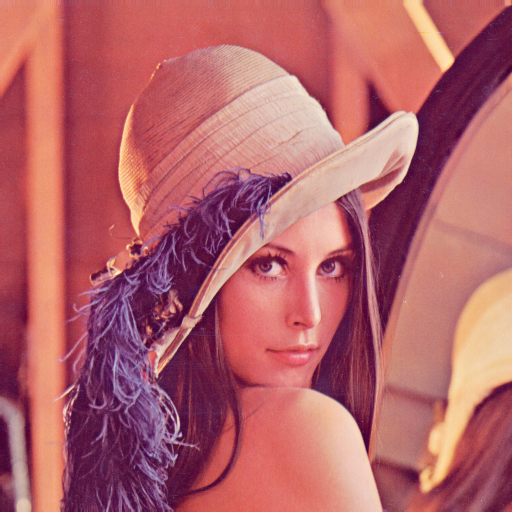
\includegraphics[width=50mm]{lenna.png}
  \caption{よく見る画像}
  \label{image:lenna}
\end{figure}

\input reference.tex

\end{document}
